We begin by providing a formal model for describing multi-agent surveillance strategy synthesis problems, in the form of a two-player game between the mobile sensors in a network and a target, in which the sensors have partial information about the target's location. 

\subsection{Multi-Agent Surveillance Game Structures}\label{sec:surveillance-games}
We define a \emph{multi-agent surveillance game structure} to be a tuple $G  = (\states,s^\init,\trans,\vis_1,\dots,\vis_n)$ where:
\begin{itemize}
\item $\states = L_s \times L_t$ is the set of states, where $L_{s} = L_1 \times L_2 \times\dots \times L_n$ is the set of joint locations of the $n$ mobile sensors, $L_i$ is the set of possible locations of sensor $i$,  and $L_t$ is the set of possible locations of the target;
\item $s^\init = (l^{\init}_1,\ldots,l^{\init}_n,l_t^\init)$ is the initial state;
\item $\trans \subseteq \states \times \states$ is the transition relation describing the possible joint moves of the sensors and the target; and
\item  $\vis_1,\dots,\vis_n$ are the \textit{visibility functions} for the $n$ sensors, where $\vis_i: L_{i} \times L_t \to \bools$ maps a state $(l_{i},l_t)$ to $\true$ iff \emph{ position $l_t$ is in the area of sight of $l_i$}.
\end{itemize}

Additionally, we define the \emph{joint visibility function} $\Vis : \states \to \bools$ that maps a state $(l,l_t)$ to $\true$ iff the set $\mathcal{I} = \{i \mid \vis_i(l_i,l_t) = \true\}$ is non-empty. Informally, $\Vis(l_s,l_t)$ is $\true$ if the target is in view of \emph{at least one} of the sensors.

\begin{figure}
\subfloat[Surveillance arena \label{fig:simple-transitions}]{
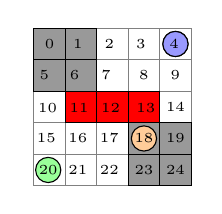
\begin{tikzpicture}[scale=0.8]
\draw[step=0.5cm,color=gray] (-1.5,-1.5) grid (1,1);
\filldraw[fill=blue,draw=black] (+0.75,+0.75) circle (0.2cm);
\filldraw[fill=red,draw=black] (0,0) rectangle (-0.5,-0.5);
\filldraw[fill=red,draw=black] (-0.5,0) rectangle (-1,-0.5);
\filldraw[fill=red,draw=black] (0,0) rectangle (0.5,-0.5);
\filldraw[fill=gray!80!white,draw=black] (-0.5,0.5) rectangle (-1,1);
\filldraw[fill=gray!80!white,draw=black] (-0.5,0) rectangle (-1,0.5);
\filldraw[fill=gray!80!white,draw=black] (-1,0.5) rectangle (-1.5,1);
\filldraw[fill=gray!80!white,draw=black] (-1,0) rectangle (-1.5,0.5);
\filldraw[fill=gray!80!white,draw=black] (0.5,-0.5) rectangle (1,-1);
\filldraw[fill=gray!80!white,draw=black] (0,-0.5) rectangle (0.5,-1);
\filldraw[fill=gray!80!white,draw=black] (0,-1) rectangle (0.5,-1.5);
\filldraw[fill=gray!80!white,draw=black] (0.5,-1) rectangle (1,-1.5);

\filldraw[fill=blue!40!white,draw=black] (+0.75,+0.75) circle (0.2cm);
\filldraw[fill=orange!40!white,draw=black] (0.25,-0.75) circle (0.2cm);
\filldraw[fill=green!40!white,draw=black]  (-1.27,-1.25) circle (0.2cm);
\node at (-1.25,+0.75) {\tiny{0}};
\node at (-0.80,+0.75) {\tiny{1}};
\node at (-0.30,+0.75) {\tiny{2}};
\node at (0.20,+0.75) {\tiny{3}};
\node at (0.73,+0.75) {\tiny{4}};
\node at (-1.33,+0.25) {\tiny{5}};
\node at (-0.85,+0.25) {\tiny{6}};
\node at (-0.35,+0.25) {\tiny{7}};
\node at (0.25,+0.25) {\tiny{8}};
\node at (0.75,+0.25) {\tiny{9}};
\node at (-1.28,-0.27) {\tiny{10}};
\node at (-0.78,-0.27) {\tiny{11}};
\node at (-0.28,-0.27) {\tiny{12}};
\node at (0.28,-0.27) {\tiny{13}};
\node at (0.75,-0.25) {\tiny{14}};
\node at (-1.3,-0.75) {\tiny{15}};
\node at (-0.8,-0.75) {\tiny{16}};
\node at (-0.3,-0.75) {\tiny{17}};
\node at (0.25,-0.75) {\tiny{18}};
\node at (0.75,-0.75) {\tiny{19}};
\node at (-1.27,-1.25) {\tiny{20}};
\node at (-0.8,-1.25) {\tiny{21}};
\node at (-0.3,-1.25) {\tiny{22}};
\node at (0.25,-1.25) {\tiny{23}};
\node at (0.75,-1.25) {\tiny{24}};
\end{tikzpicture}
\hspace{.1cm}}
%\hfill
\subfloat[Some possible transitions from the initial state in the belief-set game from Example~\ref{ex:simple-belief-game}. Note that, since the set of static sensors is empty, it is omitted from the states. For the sake of readability, some transitions are excluded.\label{fig:simple-belief-game}]{
\begin{minipage}{5.0cm}
\vspace{-2.8cm}
%{\fontsize{8}{10}\selectfont $\Vis((20,4),18) = \false,\vis(4,17) = \false,$ $\vis(4,19) = \true, \vis(4,23) = \false$}

%\smallskip

\small \[((20,4),18) \rightarrow \begin{cases}
((21,3),23) \\
((21,9),17) \\
((21,3),19) \\
((21,3),17)\\
((21,9),19)\\
((21,9),23)\\
((15,3),23) \\
((15,9),17) \\
((15,3),19) \\
((15,3),17)\\
((15,9),19)\\
((15,9),23)

\end{cases}\]

%\begin{tikzpicture}[node distance=.75 cm,auto,>=latex',line join=bevel,transform shape,scale=0.75]
%\node at (0,0) (s0) {$((20,4),18)$};
%\node  [below left of=s0,yshift=-1.5cm] (s3) {$((20,3),23)$};
%\node  [below right of=s0,yshift=-0.5cm] (s4) {$((20,9),17)$};
%\node  [left of=s3,xshift=-.35cm] (s2) {$((20,3),19)$};
%\node  [left of=s2,xshift=-.35cm] (s1) {$((20,3),17)$};
%\node  [right of=s4,xshift=.35cm] (s5) {$((20,9),19)$};
%\node  [right of=s5,xshift=.35cm] (s6) {$((20,9),23)$};
%
%\draw [->] (s0) edge (s1.north);
%\draw [->] (s0) edge (s2.north);
%\draw [->] (s0) edge (s3.north);
%\draw [->] (s0) edge (s4.north);
%\draw [->] (s0) edge (s5.north);
%\draw [->] (s0) edge (s6.north);
%\end{tikzpicture}
\end{minipage}

}
\caption{A simple surveillance game on a grid arena. Obstacles are shown in red. There are two sensors (at locations 20 and 4) coloured in blue and green respectively and the target (at location 18) is orange. The grey states are not visible to either sensor, i.e, $\Vis((20,4,l_t)) = \false$ for all grey $l_t$.}
\label{fig:simple-surveillance-game}
\vspace{-.7cm}
\end{figure}


The transition relation $T$ encodes the one-step move of the target and the $n$ sensors: First, the target makes a move, and then, the sensors move jointly in a synchronized manner. 

We denote with $T{\downarrow}i$ the projection of the transition relation $T$ on the sets of locations of the target and the sensor with index $i$. Formally, we define
$T{\downarrow }i = \{((l_i,l_t),(l_i',l_t')) \in (L_i \times L_t)^2 \mid \exists l_1,l_1',\ldots,l_{i-1},l_{i-1}',l_{i+1},l_{i+1}',\ldots,l_n,l_n' : ((l_1,\ldots,l_n,l_t),(l_1',\ldots,l_n',l_t')) \in T\}.$ 

For a state $(l_s,l_t) \in \states$ we define $\succs_t(l_s,l_t)$ to be the set of possible successor locations of the target:

$\succs_t(l_s,l_{t}) = \{l_{t}' \in L_t \mid \exists l_s'.\ ((l_s,l_t),(l_s',l_t')) \in T\}$.

We extend $\succs_t$ to sets of locations of the target by stipulating that the set $\post(l_s,L)$ consists of all possible successor locations of the target for states in $\{l_s\} \times L$. Formally, let $\post(l_s, L) = \bigcup_{l_t \in L}\succs_t(l_s,l_t)$.

For a state $(l_s,l_t)$ and a successor location of the target $l_t'$, we denote with $\succs(l_s,l_t,l_t')$ the set of successor locations of the sensors, given that the target moves to $l_t'$: 

$\succs(l_s,l_t,l_t') = \{l_s' \in L_s \mid  ((l_s,l_t),(l_s',l_t')) \in T\}$.

We assume that, for every state $s\in \states$, there exists a state $s' \in \states$ such that $(s,s') \in T$, that is, from every state there is at least one move possible (including self transitions). We also assume, that when the target moves to an invisible location, its position does not influence the possible one-step moves of the sensors. Formally, we require that if $\Vis(l_s,l_t') = \Vis(l_s,{\widehat l_t}')=\false$, then $\succs(l_s,l_t,l_t') = \succs(l_s,{\widehat l_t},\widehat{l_t}')$ for all $l_t,l_t',\widehat l_t,\widehat l_t' \in L_t$. This assumption is natural in the setting where each of the  sensors can move in one step only to locations that are in its sight.

\begin{example}\label{ex:simple-surveillance-game}
Figure~\ref{fig:simple-surveillance-game} shows an example of a multi-agent surveillance game on a grid.  The sets of possible locations $L_i$ and $L_t$ for the each of the sensors and for the target consist of the squares of the  grid. The transition relation $T$ encodes the possible one-step moves of all the sensors and the target on the grid, and incorporates all desired constraints. For example, moving to a location occupied by another sensor or the target, or to an obstacle, is not allowed.
In this example, the function $\vis_i$ encodes straight-line visibility with a range of 2: a location $l_t$ is visible to sensor $i$ from location $l_i$ if there is no obstacle on the straight line between them and the distance between the target and sensor $i$ is not larger than 2. Initially the target is not in the area of sight of the sensors, but the initial position of the target is known. However, once the target moves to one of the locations reachable in one step, in this case, locations $17,18,19 \text{ and } 23$, this might no longer be the case. More precisely, if the target moves to location $17$, then the green sensor observes its location, but if it moves to one of the other locations, then neither sensor can observe it, and its exact location will not be known. \qed
\end{example}


\subsection{Static Sensors}
We now describe a way to incorporate static sensors in the multi-agent surveillance game framework. Let $G$ be a multi-agent surveillance game structure as defined previously.  

We identify a \emph{static sensor} with a \emph{set of locations $\Lambda \subseteq L_t$ over which it operates}. 
A surveillance game can have multiple static sensors (or none). Let $\mathcal{M} = \{\Lambda_1,\dots,\Lambda_m\}$ be a given set of $m$ static sensors for $G$. For each location $l_t \in L_t$ we define  $J(l_t)$ to be the set of all indices of static sensors such that $l_t$ belongs to the corresponding set of locations, i.e, $J(l_t) = \{j \in \{1,\ldots,m\}\mid l_t\in \Lambda_j\}$. We refer to $J(l_t)$ as the set of \emph{triggered static sensors} at location $l_t$. We also define $J(L) = \bigcup_{l_t \in L} J(l_t)$ for a set of locations $L \subseteq L_t$. 

We assume that sensors do not suffer from  false positives or negatives (studying these is an avenue for future work). 
%Thus, by definition we have that the target must lie in the intersection of the state spaces of the triggered sensors, i.e., $l_t \in \bigcap_{j\in J(l_t)}\Lambda_j$. Also, when no static sensor is triggered,  then we know that the target cannot be in the union of the state spaces in which they operate, i.e, $l_t \notin \bigcup_{i=1}^m \Lambda_i$.


\subsection{Belief-Set Game Structures}\label{sec:belief-gs}

In surveillance strategy synthesis, we need to state properties of, and reason about, the information which the sensors have, i.e, the \emph{belief} about the location of the target. To this end, we can employ a powerset construction which is commonly used to transform a partial-information game into a perfect-information one, by explicitly tracking the joint knowledge of the sensors as a set of possible locations of the target. In that way we define a two-player game in which one player represents the whole sensor network, and the other player represents the target.

Given a set $A$, we denote with $\mathcal{P}(A) = \{A' \mid A'\subseteq A\}$ the powerset (set of all subsets) of $A$.

Given a  multi-agent surveillance game structure $G  = (\states,s^\init,\trans,\vis_1,\ldots,\vis_n)$ with $m$ static sensors $\mathcal{M} = \{M_{\Lambda_1},\dots,M_{\Lambda_m}\}$, we define the corresponding \emph{belief-set game structure} $G_\belief  = (\states_\belief,s^\init_\belief,\trans_\belief)$ where:
\begin{itemize}
\item $\states_\belief = L_s \times \beliefs\times \mathcal{P}(\{1,\ldots,m\})$ is the set of states, where $L_s$ is the set of joint locations of the sensors, and $\beliefs$ the set of \emph{belief sets} describing information about the location of the target, and $\mathcal{P}(\{1,\ldots,m\})$ is the set of possible sets of triggered sensors;
\item $s^\init_\belief = (l^\init_1,\ldots,l^\init_n,\{l_t^\init\},J(l_t^\init))$ as initial state;
\item $\trans_\belief \subseteq \states_\belief \times \states_\belief$ is the transition relation where $((l_s, B_t,J),(l_s', B_t',J')) \in \trans_\belief$ iff $l_s' \in  \succs(l_s,l_t,l_t')$ for some $l_t \in B_t$ and $l_t' \in B_t'$ , $J' \subseteq J(B_t')$, and one of these following conditions is satisfied:
\begin{itemize}
\item[(1)] $B_t' = \{l_t'\}$, $l_t' \in \post(l_s,B_t)$, $\Vis(l_s,l_t') = \true$;
\item[(2)] $B_t' = \{l_t' \in \post(l_s,B_t)  \mid  \Vis(l_s,l_t') = \false \} \cap \\
\phantom{B_t' = }\bigcap_{j\in J'}\Lambda_j, \text{ and } J' \neq \emptyset $;
\item[(3)] $B_t' = \{l_t' \in \post(l_s,B_t ) \mid  \Vis(l_s,l_t') = \false\}\setminus\phantom{B_t' = }\bigcup_{j=1}^m \Lambda_j$, and $J' = \emptyset$.
%\item[(1)] $B_t' = \{l_t'\}$ for some $l_t'$ such that $\vis(l_a,l_t') = \true$ and
%there exists $l_t \in B_t$ with $((l_a,l_t),(l_a',l_t')) \in \trans$;
%\item[(2)] $\begin{array}{lll}
%B_t' = \{l_t' & \mid & \vis(l_a,l_t') = \false \text{ and } \\
%&& \exists l_t \in B_t.\ ((l_a,l_t),(l_a',l_t')) \in \trans\}. 
%\end{array}
%$
\end{itemize}
\end{itemize}
Condition (1) captures the successor locations of the target that can be observed from one of the mobile sensors' current locations. Condition (2) captures the cases when the target moves to a location that cannot be observed by the mobile sensors, but triggers a non-empty set $J'$ of static sensors. Finally, condition (3) corresponds to the successor locations of the target not visible from the current location of any of the mobile sensors, and not triggering any static sensors.
%\begin{itemize}
%\item[(1)] $B_t' = \{l_t'\}$ for some $l_t'$ such that $\vis(l_a,l_t') = \true$ and
%there exists $l_t \in B_t$ with $((l_a,l_t),(l_a',l_t')) \in \trans$;
%\item[(2)] there exists $l_t \in B_t$ such that $\vis(l_a,l_t) = \true$ and 
%$\begin{array}{lll}
%B_t' = \{l_t' & \mid & \vis(l_a,l_t') = \false \text{ and } \\
%&& ((l_a,l_t),(l_a',l_t')) \in \trans\};
%\end{array}
%$
%\item[(3)] $\begin{array}{lll}
%B_t' = \{l_t' & \mid & \vis(l_a,l_t') = \false \text{ and } \\
%&& \exists l_t \in B_t: \vis(l_a,l_t') = \false \\
%&& \text{and }  ((l_a,l_t),(l_a',l_t')) \in \trans\}.
%\end{array}
%$
%\end{itemize}
%The first condition captures the successor locations of the target that can be observed from the agent's current location $l_a$. Conditions (2) and (3) correspond to belief sets consisting of all possible successor locations of the target not visible from $l_a$. In (2) those are successors of a single possible current position $l_t$ of the target that is visible from $l_a$, while in (3) the belief consist of  successors of all positions in $B_t$ not visible from $l_a$.

%\noindent{\textit{Remark}} In our model, before making a move, the agent updates its belief about the target. Thus, the belief set at each step consists of the locations the target can be in, after it moves (since it moves first). Since the target moves again immediately after the agent moves, the agent does not update its belief after it completes its own move. We note that the results in this paper can be easily extended to the case when the belief is updated after each player's move by explicitly incorporating turn-switching in the model. We choose not do so, for the sake of keeping the presentation simple.

%\begin{figure}
%\begin{center}
\begin{tikzpicture}[node distance=.9 cm,auto,>=latex',line join=bevel,transform shape,scale=.75]
\node at (0,0) (s0) {$((20,4),\{18\})$};
\node  [below left of=s0,yshift=-.5cm,xshift=-0.5cm] (s2) {$((15,3),\{19,23\})$};
\node  [below right of=s0,yshift=-.5cm,xshift=1cm] (s3) {$((15,3),\{19,23\})$};
\node  [left of=s2,xshift=-2cm] (s1) {$((15,9),\{19,23\})$};
\node  [right of=s3,xshift=2cm] (s4) {$((21,9),\{17\})$};
\draw [->] (s0) edge (s1.north);
\draw [->] (s0) edge (s2.north);
\draw [->] (s0) edge (s3.north);
\draw [->] (s0) edge (s4.north);
\end{tikzpicture}
\end{center}

%
%\vspace{-.3cm}
%\caption{Some possible transitions from the initial state in the belief-set game from Example~\ref{ex:simple-belief-game}. Since the set of static sensors is empty, it is omitted from the states. Note that, for the sake of readability, some transitions are not included.}
%\label{fig:simple-belief-game}
%\vspace{-.5cm}
%\end{figure}

\begin{example}\label{ex:simple-belief-game}
Consider the surveillance game structure from Example~\ref{ex:simple-surveillance-game}. The initial belief set is $\{18\}$, as the target's initial position is known. Figure~\ref{fig:simple-belief-game} shows some of the possible successor states of the initial state $((20,4),\{18\})$  in the belief-set game $G_\belief$.\qed
\end{example}
%After the first move of the target, there are two possible belief sets: the set $\{17\}$ resulting from the move to a location in the area of sight of the green sensor, and $\{19,23\}$ consisting of the two locations invisible to both sensors reachable in one step from location $18$.

Based on  $T_\belief$, we can define the functions $\succs_t : \states_\belief \to \mathcal{P}(\beliefs \times  \mathcal{P}(\{1,\ldots,m\}))$ and  $\succs : \states_\belief \times \beliefs \times  \mathcal{P}(\{1,\ldots,m\}) \to \mathcal{P}(L_s)$ similarly to the corresponding functions defined for $G$. 

A \emph{run} in $G_\belief$ is an infinite sequence $s_0,s_1,\ldots$ of states in $\states_\belief$, where $s_0 = s_\belief^\init$,  $(s_i,s_{i+1}) \in T_\belief$ for all $i$. 

A \emph{strategy for the target in $G_\belief$} is a function $f_t: \states_\belief^+ \to \beliefs \times \mathcal{P}(\{1,\ldots,m\})$ such that $f_t(\pi\cdot s) = (B_t, J)$ implies $(B_t ,J)\in \succs_t(s)$  for every $\pi \in \states_\belief^*$ and $s \in \states_\belief$. That is, a strategy for the target suggests a move resulting in some belief set reachable from a location in the current belief, and a set of triggered sensors.

A \emph{joint strategy for the sensors in $G_\belief$} is a function $f_s : S_\belief^+ \times \beliefs \to S_\belief$ such that, if, $f_s(\pi\cdot s,B_t,J) = (l_s',B_t,J'')$ then, $B_t' = B_t$, $J' = J$, and $l_s' \in \succs_s(s,B_t)$ for every $\pi \in \states_\belief^*$, $s \in \states_\belief$ and $B_t \in \beliefs$. Intuitively, a strategy for the sensors suggests a joint move based on the observed history of the play, the current belief about the target's position, and the set of currently triggered sensors.

The outcome of given strategies $f_s$ and $f_t$ for the sensors and the target in $G_\belief$, denoted $\outcome(G_\belief,f_s,f_t)$, is a run $s_0,s_1,\ldots$ of $G_\belief$ such that for every $i \geq 0$, we have $s_{i+1} = f_s(s_0,\ldots,s_i,B_t^i)$, where $B_t^i = f_t(s_0,\ldots,s_i)$.

\subsection{Temporal Surveillance Objectives}
We consider a set of \emph{surveillance predicates} $\SP = \{p_b \mid b \in \nats_{>0}\}$, where for $b \in \nats_{>0}$ we say that a state $(l_s,B_t)$ in the belief game structure satisfies $p_b$ (denoted $(l_s,B_t) \models p_b$) iff 
$|\{l_t \in B_t  \mid \Vis(l_s,l_t)  = \false \}| \leq b$.
%iff one of the following conditions is true:
%\begin{itemize}
%\item[(1)] $|\{l_t \in B_t \setminus \cup_i^m{\Lambda_i} \mid \Vis(l_s,l_t)  = \false, J(l_t) = \emptyset \}| \leq b$;
%\item[(2)] $|\{l_t \in B_t \cap_{j\in J}{\Lambda_j} \mid \Vis(l_s,l_t)  = \false, J(l_t) \neq \emptyset \}| \leq b$;
%\end{itemize}
%The two conditions capture the cases when there respectively are and aren't triggered static sensors. 
Intuitively, $p_b$ is satisfied by the states in the belief game structure where the size of the belief set does not exceed the threshold $b \in \nats_{>0}$.

We study surveillance objectives expressed in a fragment  of linear temporal logic (LTL) over surveillance predicates.  We consider  \emph{safety surveillance objectives} expressed using the temporal operator $\LTLglobally$ and \emph{liveness surveillance objectives} expressed using the temporal operators $\LTLglobally$ and $\LTLeventually$.

A \emph{safety surveillance objective} $\LTLglobally p_b$ requires that the size of the belief-set never exceeds the given threshold $b$. More formally, an infinite sequence of states $s_0,s_1,\ldots$ in $G_\belief$ satisfies the safety property $\LTLglobally p_b$ if and only if for every $i\geq 0$ it holds that $s_i \models p_b$.  A \emph{liveness surveillance objective} $\LTLglobally\LTLfinally p_b$, on the other hand, requires that 
the size of the belief is smaller or equal to the bound $b$  infinitely often. That is, $s_0,s_1,\ldots$ in $G_\belief$ satisfies $\LTLglobally\LTLfinally p_b$ if for every $i \geq 0$ there exists $j >i$ such that $s_j\models p_b$. 

In this paper we consider safety and liveness surveillance objectives, as well as conjunctions of such objectives. We remark the following equivalences of surveillance objectives:
\begin{itemize}
\item $\LTLglobally p_a \wedge \LTLglobally p_b \equiv \LTLglobally p_{\min{(a,b)}}$;
\item $\LTLglobally\LTLfinally p_a \wedge \LTLglobally\LTLfinally p_b \equiv \LTLglobally\LTLfinally p_{\min{(a,b)}}$;
\item if $a \leq b$, then $\LTLglobally p_a \wedge \LTLglobally\LTLfinally p_b \equiv\LTLglobally p_a$. 
\end{itemize}
Using these equivalences, we can restrict our attention to surveillance objectives of one the following  forms: $\LTLglobally p_b$, $\LTLglobally\LTLfinally p_b$ or $\LTLglobally p_a \wedge \LTLglobally\LTLfinally p_b$, where $a > b$. 
 


%\begin{example}
%We can specify that the sensors are required to always know with certainty the location of the target as
%$\LTLglobally p_1$.
%A more relaxed requirement is that the sensors' uncertainty never grows above $5$ locations, and is infinitely often reduced to at most $2$ locations: $\LTLglobally p_5 \wedge \LTLglobally\LTLfinally p_2$.
%\qed
%\end{example}


%\subsection{Incorporating Task Specifications}
%We can integrate LTL objectives not related to surveillance, i.e., \emph{task specifications}, by considering, in addition to $\SP$, a set $\AP$ of atomic predicates interpreted over states of $G$. In order to define the semantics of $p \in \AP$ over states of $G_\belief$, we restrict ourselves to predicates observable by the agent. 
%Formally, we require that for $p \in \AP$, and states $(l_a,l_t')$ and $(l_a,l_t'')$ with $\vis(l_a,l_t')=\vis(l_a,l_t'')=\false$ it holds that $(l_a,l_t') \models p$ iff $(l_a,l_t'') \models p$. One class of such predicates are those that depend only on the agent's position.

%\begin{example}
%Suppose that $\mathit{at\_goal}$ is a predicate true exactly when the agent is at some designated goal location. We can then state that the agent visits the goal infinitely often while always maintaining belief uncertainty of at most $10$ locations using the LTL formula $\LTLglobally\LTLfinally \mathit{at\_goal} \wedge \LTLglobally p_{10}$.
%\qed
%\end{example}

\subsection{Multi-Agent Surveillance Synthesis Problem}
A \emph{multi-agent surveillance game} is a triple $(G,\mathcal M,\varphi)$, where $G$ is a surveillance game structure, $\mathcal M$ is a set of static sensors,  and $\varphi$ is a surveillance objective. A \emph{winning strategy for the sensors for $(G,\mathcal M,\varphi)$} is a joint strategy $f_s$ for the sensors in the corresponding belief-set game structure $G_\belief$ such that for every strategy $f_t$ for the target in $G_\belief$ it holds that $\outcome(G_\belief,f_s,f_t) \models \varphi$. Analogously, a \emph{winning strategy for the target for $(G,\mathcal M,\varphi)$} is a strategy $f_t$ such that, for every strategy $f_s$ for the mobile sensors in $G_\belief$, it holds that $\outcome(G_\belief,f_s,f_t) \not\models \varphi$.

{\textit{\textbf{Problem statement: }}} Given a multi-agent surveillance game $(G,\mathcal M,\varphi)$,  compute a joint strategy for the mobile sensors that is winning for the game $(G,\mathcal M,\varphi)$.

In the remainder of the paper we show how to solve the multi-agent surveillance synthesis problem in a compositional manner.  The key idea is to decompose the problem into a set of single-sensor surveillance games over smaller sets of locations, and solve each of these games separately. 

